\chapter{Description détaillée du projet}
\section*{Introduction}
Dans ce chapitre nous allons présenter le projet de façon détaillée, nous expliquerons chaque fonction du système dont la fonction qui m'a été confiée lors de mon stage.

\section{Système de recharge automatique sans fil AWC}
Comme on a pu voir précédemment, PRIMOVE de BOMBARDIER a décidé de réaliser un système de recharge automatique sans fil se basant sur le principe de transfert d’énergie par induction. Pour mieux appréhender le système, on se propose d’expliquer chaque fonction du système AWC.

\begin{figure}[H]
 \centering
 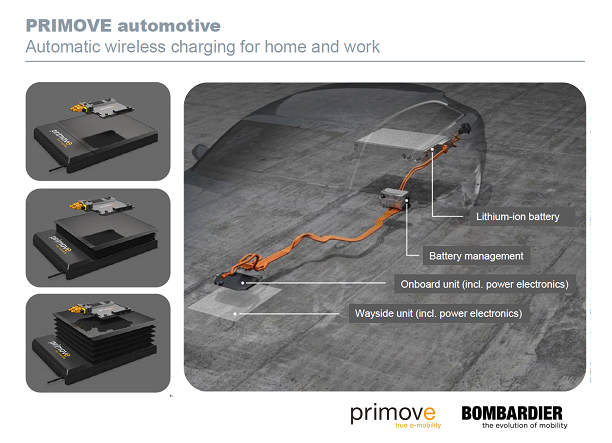
\includegraphics[scale=1]{images/look_through_awc}
 \caption{Système AWC}
\end{figure}

Le but du système AWC est de transférer de l’énergie électrique sans fil au véhicule. Ce transfert d’énergie atteint un niveau d’efficacité très haut grâce aux deux composants principaux du système le WSD (Wayside subsystem) qui est la partie statique installé sur la chaussée et connecté au réseau électrique et le deuxième composant le ORU (Onboard Receiving Unit) qui est la partie reliée au véhicule. Le système est équipé d’un logiciel embarqué basé sur le FrameWork AutoSar pour pouvoir gérer toutes les fonctionnalités du système.

Le système AWC est composé de plusieurs fonctions : 

\begin{itemize}
\item Les machines à états ORU et Wayside.
\item La fonction de Positionnement POS.
\item Z-Mover.
\item Transfert d’énergie.
\item Détecteur de métal (Foreign Objet Detection FOD).
\item L’interface Homme-Machine.
\item Fonction d’indication d’état LED.
\item Protection.
\item Communication.
\item Diagnostique.
\item Sécurité.
\end{itemize}

\begin{figure}[H]
 \centering
 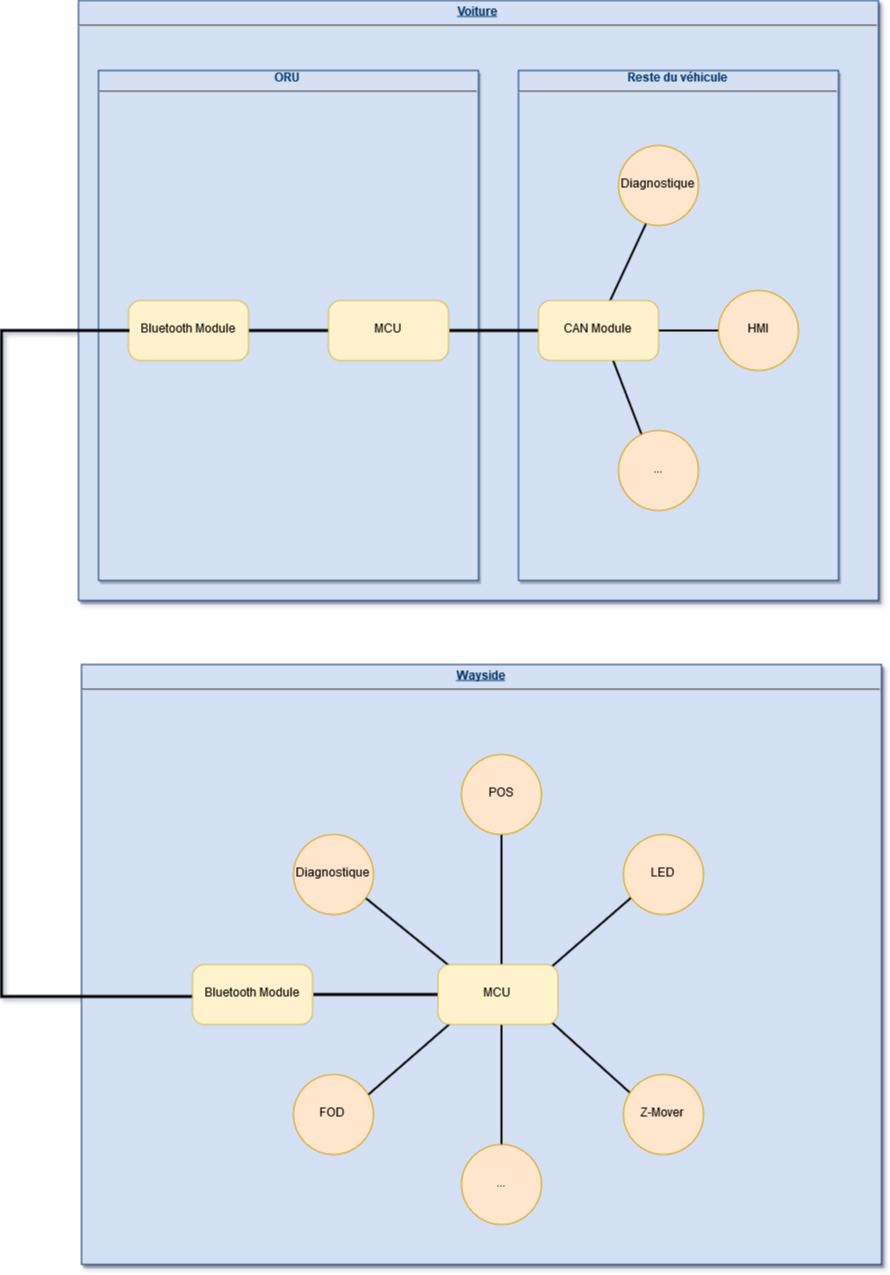
\includegraphics[scale=0.4]{images/arch_awc}
 \caption{Architecture générale AWC}
\end{figure}

Afin de pouvoir commencer le chargement du véhicule, ce dernier doit être bien positionné au-dessus du Wayside. Un système de positionnement POS est mis à disposition pour aider le conducteur à bien se positionner en affichant la position relative du véhicule au Wayside.

\begin{figure}[H]
 \centering
 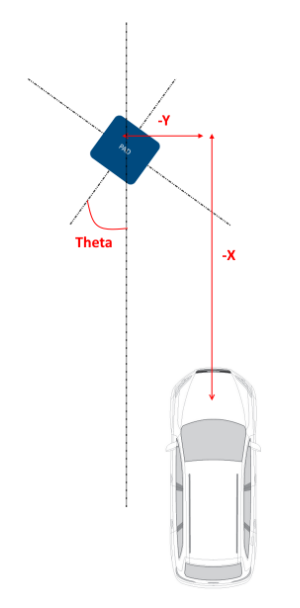
\includegraphics[scale=0.7]{images/pos}
 \caption{Fonction POS}
\end{figure}

Les objets métalliques atteindre des températures très haute à cause du champs électromagnétique généré par le système. Donc pour des raisons de sécurité, après avoir bien positionné le véhicule au-dessus du Wayside, le système doit vérifier qu’aucun objet métallique se trouve entre l’ORU et le Wayside, pour cela on fait appel au FOD (Foreign Object Detection) ou bien le détecteur d’objet métallique. Ce composant incorporé dans le Wayside permet de détecter les objets métalliques présents au-dessus de lui de distance de 40 millimètres.

\begin{figure}[H]
 \centering
 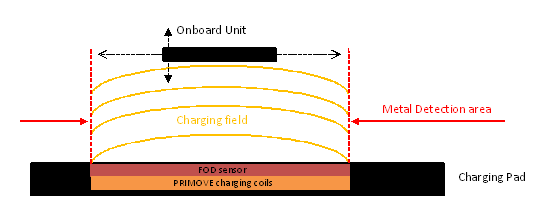
\includegraphics[scale=1]{images/fod_awc}
 \caption{Fonction FOD}
\end{figure}

Quand le système détecte que le champ est clair, il procède à l’étape suivante qui est de soulever la plateforme du Wayside contenant la bobine permettant le chargement du véhicule. Cette étape est primordiale car elle permet au système de réduire la distance entre la bobine principale et secondaire, et par conséquent réduire les pertes du champ magnétique. Le composant responsable de cette action est le Z-Mover, il est à nouveau baissé à la fin du chargement.

\begin{figure}[H]
 \centering
 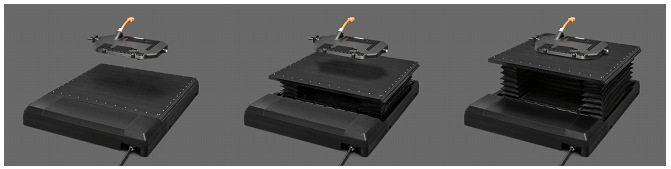
\includegraphics[scale=0.8]{images/zmover_awc}
 \caption{Fonction Z-Mover}
\end{figure}

Pendant le chargement du véhicule intervient la fonction « Protection » du système, qui responsable de désactiver le transfert d’énergie si elle détecte un surplus en tension ou en courant, elle peut aussi diminuer le montant d’énergie transféré quand le système surchauffe.

Pour assurer la communication et la transmission constante d’information entre le Wayside et l’ORU, le système a recours au WCAN (Wireless CAN). Il permet aux deux composants de s’échanger des informations nécessaires pour le bon déroulement du chargement telles que la position du véhicule par rapport au Wayside, la détection d’objet métallique et bien d’autres. La fonction « Sécurité » s’occupe de s’assurer de l’exactitude de l’information transmise via WCAN et de l’identité de l’expéditeur, afin d’éviter toutes mauvaises manipulations et attaques sur le système.

L’interface Homme Machine permet au conducteur de configurer le système AWC tel que se connecter à un Wayside, entrer le code PIN, changer le nom du Wayside…. Elle permet aussi d’assister le conducteur lors du positionnement du véhicule en lui affichant sa position relative au Wayside.

La fonction « LED » indique l’état actuel du système AWC à travers une LED multi couleur placée sur le Wayside.

\section{Fonction Sécurité}

Afin de minimiser la probabilité d'une mauvaise utilisation des fonctions du système AWC, la fonction sécurité intervient pour rendre le système robuste.

\subsection{Couche de sécurité}

Ce concept de sécurité est réparti en plusieurs couches de mise en œuvre et il est illustré dans la figure suivante : 

\begin{figure}[H]
 \centering
 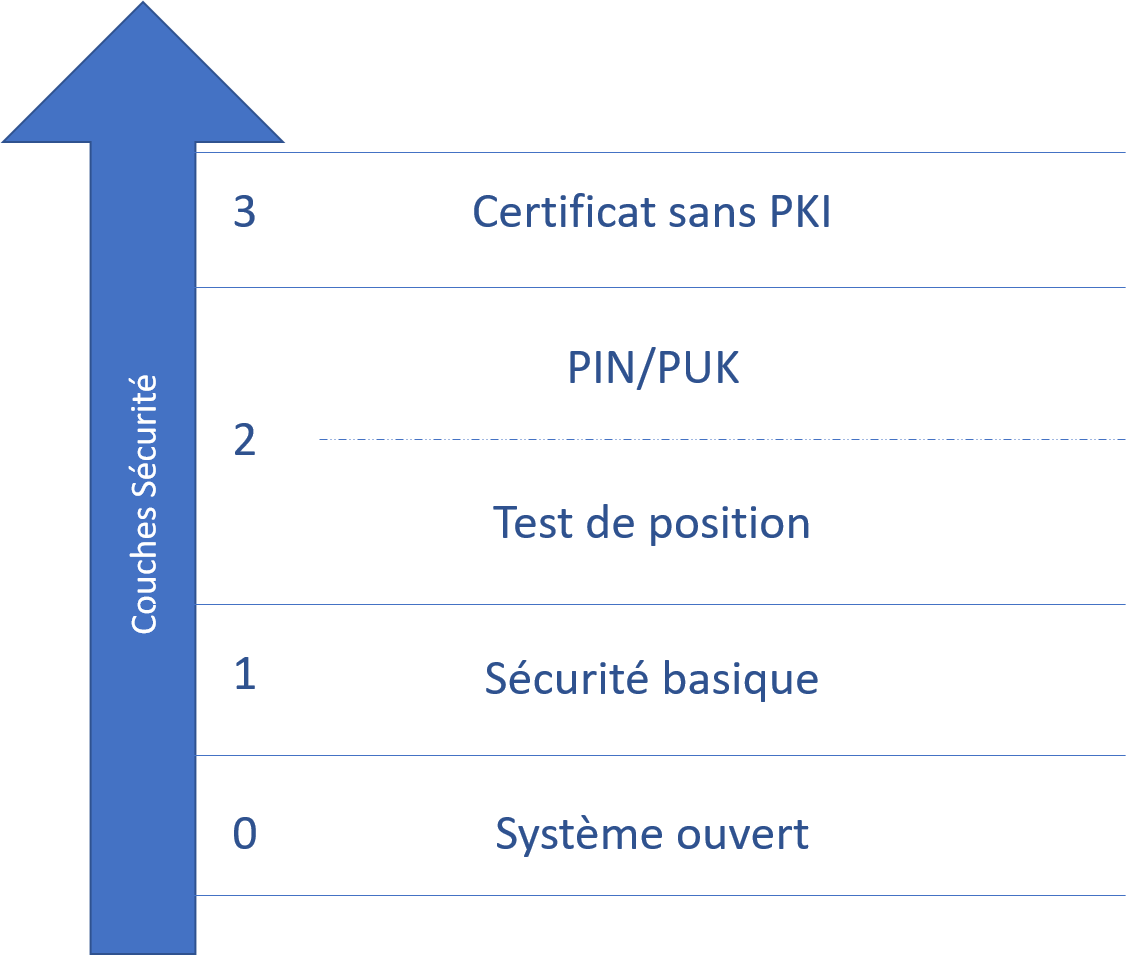
\includegraphics[scale=0.8]{images/security_layers}
 \caption{Couches concept de sécurité}
\end{figure}

La couche sécurité niveau zéro définit un système ouvert sans aucune mesure de sécurité, alors que la couche de niveau un implémente un mécanisme de sécurité permettant la connexion au Wayside à travers le Bluetooth Low Energy BLE avec un code qui est fixe.

En plus des mesures de sécurité implémentées dans la couche une, la sécurité du niveau deux nous donne le droit de changer le code utilisé lors de la connexion au Wayside, elle ajoute aussi un mécanisme de sécurité qui ne permet au véhicule de se connecter au Wayside que quand il est bien positionné au-dessus de ce dernier. On peut dire que la couche de sécurité de niveau deux est une extension de celle du niveau un.

La différence la plus frappante entre la dernière couche et l'avant dernière est l'utilisation de la fonctionnalité PIN/PUK. La couche de sécurité de niveau deux utilise le code PIN/PUK pour l'autorisation. Alors que la couche de sécurité de niveau trois doit utiliser le code PIN/PUK pour l'authentification (autorisation spécifique à l'utilisateur). La dernière couche est encore en phase de développement.

Le système Automatic Wireless Charging est donc implémenté avec la couche sécurité de niveau deux.

\subsection{Couche sécurité niveau deux}

Ce concept de sécurité est divisé en plusieurs sous-projets : 

\begin{itemize}

	\item Protocole PIN/PUK.
	\item Protocole d'appariement.
	\item Protocole de mise à jour de clé
	\item Protocole d'établissement d'une connexion sécurisée.
	\item Protocole de suppression d'appariement.
	\item Protocole de changement de PIN.

\end{itemize}

\subsubsection{Protocole PIN/PUK}

Dans le processus d'authentification des points d'extrémité, les autorisations doivent être obtenues par la méthode SRP (Secure Remote Password), dans laquelle aucune mémoire sécurisée (aucun HSM) n'est disponible pour les points d'extrémité.

Le but de ce protocole PIN/PUK est d'établir un secret partagé commun pour deux partenaires de communication.

En plus de ce protocole, ce secret commun doit être utilisé pour vérifier si les deux partenaires de communication PIN/PUK sont connus ou non, ainsi que pour acheminer les autres messages au bon partenaire ceci prévient les attaques MITM (Man In The Middle).

La méthode SRP (Secure Remote Password) a besoin de plusieurs paramètres\footnote{Valeur pour chaque paramètre dans les annexes} : 

\begin{itemize}

	\item N : Nombre premier 
	\item g : Générateur
	\item s : Salt
	\item I : Username ou bien Identify
	\item P : Mot de passe = PIN/PUK
	\item V : Vérifiant
	\item k : Multipliant
	\item B : La clé publique du Wayside
	\item b : La clé privée du Wayside
	\item A : La clé publique de l'ORU
	\item a : La clé privée de l'ORU
	\item u : Paramètre aléatoire

\end{itemize}

Pour le fonctionnement, l'utilisateur entre le PIN/PUK à travers l'interface Homme-Machine IHM, (si c'est la première connexion au Wayside, le PIN par défaut est "000000"), si le PIN est correct, l'ORU se connecte au service d'appariement du Wayside et crée une clé de session symétrique commune (SKSRP Common Symmetrical Session Key) selon le protocole SRP en utilisant le PIN comme mot de passe.

Si le système détecte que le code entré par l'utilisateur est bel et bien le PUK, il lui donne accès à l'espace d'administration du Wayside où il peut flasher ce dernier ou bien changer son code PIN.

\subsubsection{Protocole d'appariement}

Le véhicule ou bien l'ORU pour être exact, doit initier le processus d'appariement en envoyant une demande au Wayside. Une fois l'orientation et la position du véhicule sont correctes, on utilise l'authentification PIN/PUK pour créer une clé de session SKSRP qui sera utilisée dans le processus d'appariement.

La figure suivante résume ce processus : 

\begin{figure}[H]
 \centering
 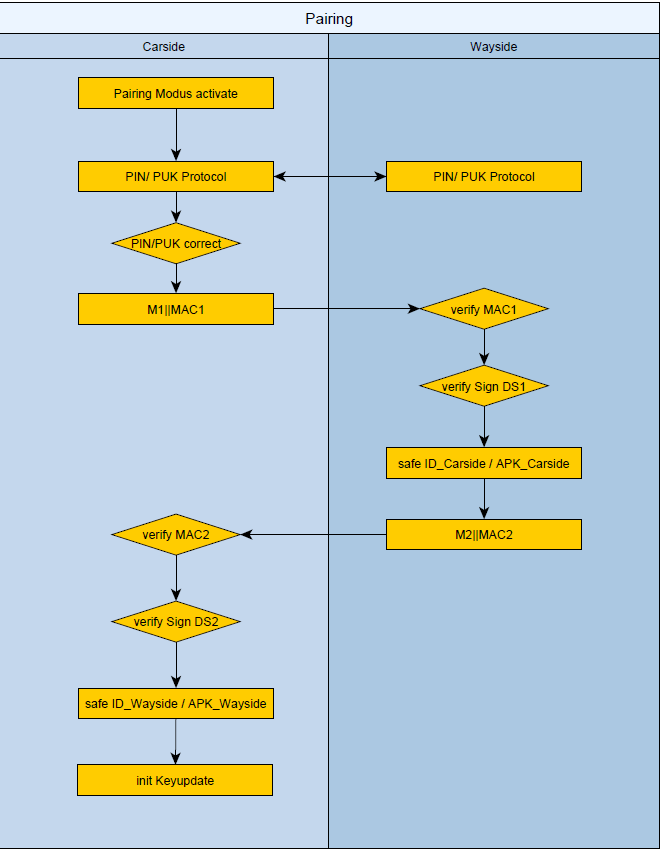
\includegraphics[scale=0.6]{images/pairing_process}
 \caption{Processus d'appariement}
\end{figure}

Avant de commencer le processus d'appariement, le véhicule doit être bien orienté et positionné : 

\begin{itemize}

	\item La vitesse du véhicule est 0 Km/h.
	\item Aucun métal détecté entre l'ORU et le Wayside.

\end{itemize}

Après l'authentification PIN/PUK, l'ORU commence par regrouper son ID, sa clé publique et sa signature dans un message \textbf{M1} et le transmet au Wayside sécurisé par MAC (Message Authentication Code).

Lors de la réception de \textbf{M1}, le Wayside vérifie la signature du message à l'aide de la clé publique de l'ORU, et stocke de façon permanente son ID dans une liste "Appareil de confiance" TDL (Trusted device).

Même chose mais de façon inverse, le Wayside envoie ses données à l'ORU qui les teste pour stocker l'ID du Wayside dans sa liste à lui.

Une fois le processus d'appariement fini, on commence le processus de mise à jour de clé.


